\subsection{Deformable Bodies}
\label{sec:deformable}

Our method naturally extends to support frictional contact involving deformable
bodies. In this experiment, we simulate deformable FinRay gripper fingers
attached to a Panda arm in a peg-in-hole task (Fig.
\ref{fig:finray}). Each finger is discretized as a
tetrahedral mesh with 1,009 vertices and 2668 tetrahedra and simulated with the
linear corotational model described in \cite{bib:han2023}.
The fingers are attached to the Panda hand using holonomic constraints between
the mesh vertices the rigid hand. Material properties of the fingers include
a Young's modulus of $E=2.5 \times 10^6$ Pa, Poisson's ratio $\nu=0.49$, density
$\rho=1000$ kg/m$^3$, and Rayleigh stiffness damping coefficient $\zeta=0.01$ s.

The robot is teleoperated using a 6-DoF space mouse to control the end-effector
pose, while the arm's joint positions are solved through differential inverse
kinematics. The simulation employs the Lagged approximation with a 10 ms time
step. The robot is commanded to place a rigid cylinder into a rigid utensil
holder welded to the table. The average simulation time per time step is 24.5
ms, fast enough for interactive teleoperation, and the maximum and average
number of contact constraints are 114 and 73.9, respectively. 

\begin{figure}[!h]
    \centering
    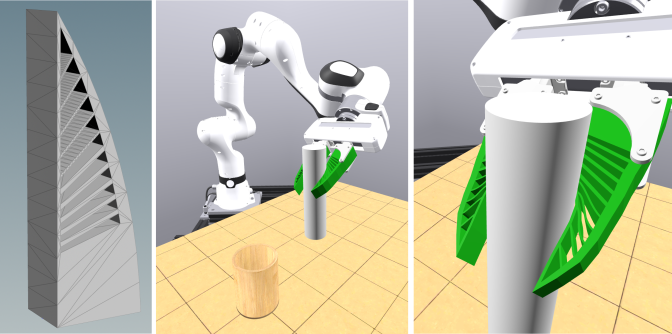
\includegraphics[width=\columnwidth]{figures/TestCases/Deformable/combined.png}
    \caption{Simulation of deformable Finray grippers in a teleoperation task. (Left)
    the mesh used to model the FinRay gripper. (Center) the peg-in-hole teleoperation
    task. (Right) the characteristic caging deformation induced by frictional contact
    with the manipuland.}
    \label{fig:finray}
\end{figure}
